\documentclass{article}
%%!TEX encoding = UTF-8 Unicode
\usepackage[utf8]{inputenc}
%\usepackage{ngerman}
%\usepackage[ps2pdf,a4paper,colorlinks]{hyperref}
%\usepackage[a4paper,colorlinks]{hyperref}
\usepackage[a4paper]{hyperref}
\usepackage[a4paper,%
	inner=3.5cm,%
	outer=3.5cm,%
	top=4cm,%
	bottom=4cm,%
	marginparwidth=2.5cm,%
	marginparsep=0.3cm,%
	includehead]{geometry}
\usepackage{makeidx}
\usepackage[nottoc,numbib]{tocbibind}
\usepackage[fleqn]{amsmath}
\usepackage{amsthm}
\usepackage{amstext}
\usepackage{amssymb}
\usepackage{mathtools}
\usepackage{xparse}
\usepackage{tikz}
\usetikzlibrary{automata,positioning}
% doesnt work?
%\usepackage{vaucanson-g}

\hypersetup{%
	pdftitle = {Language Operations and a Structure Theory of ω-Languages},%
	pdfsubject = {},%
	pdfauthor = {Albert Zeyer}%
}

% funktioniert nicht?
%\makeidx

%!TEX root =  index.tex

% some useful stuff:
% http://www.automata.rwth-aachen.de/material/skripte/latex/latex.pdf
% http://en.wikibooks.org/wiki/LaTeX/Mathematics
% http://en.wikibooks.org/wiki/LaTeX/Advanced_Mathematics
% http://en.wikibooks.org/wiki/LaTeX/Theorems

\newtheorem{thm}{Theorem}[section]
\newtheorem{lem}[thm]{Lemma}

\theoremstyle{plain}\newtheorem{lemma}{Lemma}[section]
\theoremstyle{plain}\newtheorem{theorem}[lemma]{Theorem}
\theoremstyle{definition}\newtheorem{mydef}[lemma]{Definition}
\theoremstyle{definition}\newtheorem{algo}[lemma]{Algorithm}
\theoremstyle{plain}\newtheorem{example}[lemma]{Example}

\newcommand{\K}{\mathcal{K}}
\newcommand{\Reg}{\text{Reg}}
\newcommand{\Lang}{\mathcal{L}}
\newcommand{\A}{\mathcal{A}}
\newcommand{\T}{\mathcal{T}}
\newcommand{\F}{\mathcal{F}}
\newcommand{\Q}{\mathbb{Q}}
\newcommand{\R}{\mathbb{R}}
\newcommand{\N}{\mathbb{N}}
\newcommand{\B}{\mathbb{B}}
\newcommand{\Power}{\mathcal{P}}

\newcommand{\mathtext}[1]{\textup{\textrm{#1}}}
\newcommand{\PT}{\mathtext{PT}}
\newcommand{\LT}{\mathtext{LT}}

% got some help here: http://tex.stackexchange.com/questions/13554/define-something-like-lim-but-for-another-name

\newcommand{\ext}{\operatorname{ext}}
\newcommand{\Inf}{\operatorname{Inf}}
\newcommand{\BC}{\operatorname{BC}}
\newcommand{\dext}{\operatorname{\overline{ext}}}
\newcommand{\dlim}{\operatorname{\overline{lim}}}
\newcommand{\Kleene}{\operatorname{\widehat{Kleene}}}
\newcommand{\limClosure}{\operatorname{\widehat{lim}}}
\newcommand{\Occ}{\operatorname{Occ}}
\newcommand{\existsinf}{\exists^\omega}
\newcommand{\overx}{\overset{\times}}
%\newcommand{\overx}{\stackrel{\times}}
\newcommand{\Ax}{\overx{\A}}
\newcommand{\Langreg}{\Lang^*(\text{reg})}
\newcommand{\LangOreg}{\Lang^\omega(\text{reg})}

\newcommand{\defword}[1]{{\bf #1}}

% inspired by http://ftp.fernuni-hagen.de/ftp-dir/pub/mirrors/www.ctan.org/macros/latex/contrib/braket/braket.sty
\def\mid@vertical{\mskip1mu\vrule\mskip1mu}
\def\midvert{\egroup\;\mid@vertical\;\bgroup}
\NewDocumentCommand\Set{mg}{%
    \IfNoValueTF{#2}{%
        \ensuremath{\left\{ #1 \right\}}%
    }{%
        \ensuremath{\left\{ {#1} \;\mid@vertical\; {#2} \right\}}%
    }%
}

%\newcommand{\SetS}[1]{\bigl\{ #1 \bigr\}}
%\newcommand{\SetC}[2]{\bigl\{ #1 \bigm| #2 \bigr\}}
%\DeclarePairedDelimiterX\SetC[2]{\lbrace}{\rbrace}{ #1 \,\delimsize|\, #2 }

%\newcommand{\abs}[1]{\mathopen| #1 \mathclose|}
%\newcommand{\Abs}[1]{\left| #1 \right|}
\newcommand{\abs}[1]{\left| #1 \right|}

% http://de.wikibooks.org/wiki/LaTeX-W%C3%B6rterbuch:_today
\def\monthgerman{\ifcase\month \or
  Januar\or Februar\or M\"arz\or April\or Mai\or Juni\or
  Juli\or August\or September\or Oktober\or November\or Dezember\fi}
\def\todaygerman{\number\day.~\monthgerman\space\number\year}


\begin{document}
\title{Language Operations and a Structure Theory of $\omega$-Languages}
\author{Albert Zeyer}
%\date{10. Februar 2011}
\date{\today}

\maketitle
\tableofcontents

%!TEX root =  index.tex

\section{Introduction}

The study of formal languages and finite-state automata theory is very old and fundamental in theoretical computer science. Regular expressions were introduced by Kleene in 1956 (\cite{Kleene56}). Research on the connection between formal languages, automata theory and mathematical logic began in the early 1960's by Büchi (\cite{Buchi60}). Good introductions into the theory are \cite{FinAutLogR109} and \cite{LangAutLogicR102}.

We call languages over finite words the $*$-languages. Likewise, $\omega$-languages are over infinite words.

The class of regular $*$-languages is probably the most well studied language class. Its expressiveness is exactly equivalent to the class of finite-state automata as well as regular expressions. For many applications, less powerful subsets of the regular $*$-languages are interesting, like starfree $*$-languages, locally testable $*$-languages, etc., as well as more powerful supersets, like context-free $*$-languages.

The research on $\omega$-languages and their connection to finite-state automata began a bit later by Büchi \cite{DecisionSOR111} and \cite{Muller63}. As for the $*$-languages, the most well studied $\omega$-language class are the regular $\omega$-languages. Good introductions into these theories are \cite{AutInfObjsR103}, \cite{InfCompR101}, \cite{OmLangR108} and \cite{InfWordsR110}.

The acceptance-condition in automata for $*$-languages is straight-forward. If we look at $\omega$-languages, several different types of automata and their acceptance have been thought of, like Büchi-acceptance or Muller-acceptance, or E-acceptance and A-acceptance.

For all types, we can also argue with equivalent language-theoretical operators which operate on a $*$-language and transform them into an $\omega$-language. We will study the equivalences in more detail. The most important operators are $\ext$, $\lim$ and boolean combinations of those.

Depending on the $* \rightarrow \omega$ language operator or the $\omega$-automaton acceptance condition, we get different $\omega$-language classes. This was studied earlier already in detail for the class of regular $*$-languages. E.g., we get the result $\BC \ext \Langreg \subsetneqq \BC \lim \Langreg$ and $\lim \cap \dlim \Langreg = \BC \ext \Langreg$. In terms of $\omega$-automata, that is that boolean combinations of E-automata are strictly less powerful than boolean combinations of deterministic Büchi automata. Those in turn are equivalent to Muller automata.

When we look at other $*$-language classes, like starfree $*$-languages and the different ways to transform them into $\omega$-languages, we can get different results. E.g., $\BC \ext \Lang(\PT) = \BC \lim \Lang(\PT)$. This study is the main topic of this thesis.

\section{Background results on regular $\omega$-languages}

\subsection{Preliminaries}
We introduce some common terminonoly used in this thesis.

The set of natural numbers $1,2,3,\dots$ is denoted by $\N$, likewise $0,1,2,3,\dots$ by $\N_0$.

An \defword{alphabet} is a finite set of \defword{symbols}. We usually denote an alphabet by $\Sigma$ and its elements by $a, b, c, \dots$. A finite sequence of elements in $\Sigma$ is also called a \defword{finite word}, often named $u, v, w, \dots$. The set of such words, including the \defword{empty word} $\epsilon$, is denoted by $\Sigma^*$. Likewise, $\Sigma^+$ is the set of non-empty words. Infinite sequences over $\Sigma$ are called \defword{infinite words}, often named $\alpha, \beta$. The set of such infinite words is denoted by $\Sigma^\omega$.

A subset $L \subseteq \Sigma^*$ is called a \defword{language} of finite words or also called a \defword{$*$-language}. Likewise, a subset $L^\omega \subseteq \Sigma^\omega$ is called an \defword{$\omega$-language}.

A set $\Lang$ of $*$-languages is called a \defword{$*$-language class}. Likewise, a set $\Lang^\omega$ of $\omega$-languages is called a \defword{$\omega$-language class}.

We can \defword{concatenate} finite words with each other and also finite words with infinite words. For languages $L_1 \subseteq \Sigma^*$, $L_2 \subseteq \Sigma^*$, $L^\omega_3 \subseteq \Sigma^\omega$, we define the concatenation $L_1 \cdot L_2 := \Set{v \cdot w}{v \in L_1, w \in L_2}$ and $L_1 \cdot L^\omega_3 := \Set{v \cdot \alpha}{v \in L_1, \alpha \in L^\omega_3}$. Exponentation of languages is defined naturally: For $L \subseteq \Sigma^*$, we define $L^0 := \Set{\epsilon}$ and $L^{i+1} := L^i \cdot L$ for all $i \in \N_0$. The union of all such sets, is called the \defword{Kleene closure} or the \defword{Kleene star} operator, defined as $L^* := \cup_{i\in\N_0} L^i$. The \defword{positive Kleene closure} is defined as $L^+ := \cup_{i\in\N} L^i$. The \defword{infinite Kleene closure} is defined by $L^\omega := \Set{w_1 \cdot w_2 \cdot w_3 \cdots}{w_i \in L}$.

\subsection{The class of regular $*$-languages}

A \defword{regular expression} is representing a language over an alphabet $\Sigma$. Regular expressions are defined recursively based on the ground terms $\emptyset$, $\epsilon$ and $a$ for $a \in \Sigma$ denoting the languages $\emptyset$, $\Set{\epsilon}$ and $\Set{a}$. Then, if $r$ and $s$ are regular expressions representing $R, S \subseteq \Sigma^*$, then also $r+s$ (written also as $r|s$, $r \vee s$, $r \cup s$), $r s$ (written also as $r \cdot s$) and $r^*$ are regular expressions, representing $R \cup S$, $R \cdot S$ and $R^*$. Let $\Lang^*(\text{RE})$ be the set of languages which can be represented as regular expressions.

We extend these expression also by $r \wedge s$ (written also as $r \cap s$) and $-r$ (written also as $\neg r$), representing the language $R \cap S$ and $-R := \Set{w \in \Sigma^*}{w \not\in R}$. Some basic result of the study of formal languages, as can be seen in e.g. \cite{FinAutLogR109}, is the equivalence of the class of these extended regular expression languages and $\Lang^*(\text{RE})$.

A \defword{non-deterministic} \defword{finite-state automaton} $\A$ over an alphabet $\Sigma$ is given by a finite set $Q$ of \defword{states} and a subset $\Delta \subseteq Q \times \Sigma^* \times Q$ of \defword{transitions}. In most cases we also have an \defword{initial states} $q_0 \in Q$ and a subset $F \subseteq Q$ of \defword{final states}.

We write:
\[ \A = (Q, \Sigma, q_0, \Delta, F). \]

The automaton is \defword{deterministic} (a DFA) iff $\Delta$ is a function $Q \times \Sigma \rightarrow Q$. In that case, we often call the function $\delta$.

Two transitions $(p,a,q), (p',a',q') \in E$ are \defword{consecutive} iff $q=p'$.

A \defword{run} in the automaton $\A$ is a finite sequence of consecutive transitions, written as:
\[ q_0 \xrightarrow{a_0} q_1 \xrightarrow{a_1} q_2 \dots \]

An automaton $\A = (Q, \Sigma, q_0, \Delta, F)$ \defword{accepts} a finite word $w = (a_0,a_1,...,a_n) \in \Sigma^*$ iff there is a run $q_0 \rightarrow^{a_0} q_1 \rightarrow^{a_1} q_2 \dots \rightarrow^{a_n} q_{n+1}$ with $q_0 \in I$ und $q_{n+1} \in F$.

The $*$-language $L^*(\A)$ is defined as set of all finite words which are accepted by $\A$.

The set of $*$-languages accepted by a NFA is called $\Lang^*(\text{NFA})$. Likewise, $\Lang^*(\text{DFA})$ is the set of $*$-languages accepted by a DFA. A basic result (see for example \cite{FinAutLogR109} or \cite{InfWordsR110}) is
\[ \Lang^*(\text{DFA}) = \Lang^*(\text{NFA}) = \Lang^*(\text{RE}) . \]

This class of $*$-languages is called the class of \defword{regular $*$-languages}. We name it $\Langreg$ from now on.

\subsection{The class of regular $\omega$-languages}
\label{reg-omega-lang}

The class of regular $\omega$-languages can be defined in many different ways. We will use one common definition and show some equivalent descriptions.
\[ \LangOreg := \Set{ \bigcup_i\ U_i \cdot V_i^\omega }{ U_i, V_i \in \Langreg } \]

A different, very common description is in terms of automata.

An automaton $\A = (Q, \Sigma, E, I, F)$ \defword{Büchi-accepts} a word $\alpha = (a_0,a_1,a_2,...) \in \Sigma^\omega$ iff there is an infinite run $q_0 \rightarrow^{a_0} q_1 \rightarrow^{a_1} q_2 \rightarrow^{a_2} q_3 ...$ with $q_0 \in I$ and $\{ q_i | q_i \in F \}$ infinite, i.e. which reaches a state in $F$ infinitely often.

The language $L^\omega(\A)$ is defined as the set of all infinite words which are Büchi-accepted by  $\A$.

An automaton $\A$ is a Büchi automaton iff we use the Büchi-acceptence.

A basic result of the study of this language class is: The set of all languages accepted by a non-deterministic Büchi automaton is exactly $\LangOreg$ (see \cite{InfCompR101} or others). %S218
Deterministic Büchi automata are less powerful, e.g. they cannot recognise $(a+b)^* b^\omega$.

There are some different forms of $\omega$-automata which differ in their acceptance condition. Noteable are the \defword{Muller conition}, the \defword{Rabin condition}, the \defword{Streett condition} and the \defword{Parity condition}. With such an acceptance condition, we call it \defword{Muller automaton}, etc. The main theorem of deterministic $\omega$-automata states:
\begin{itemize}
\item Non-deterministic Büchi automata,
\item a boolean combination of deterministic Büchi automata,
\item deterministic Muller automata,
\item deterministic Rabin automata,
\item deterministic Streett automata
\item deterministic Parity automata
\end{itemize}
all recognize the same languages. See \cite{InfCompR101}, \cite{LangAutLogicR102}, \cite{InfWordsR110} and others. Part of it is the \defword{McNaughton's Theorem} which states the equivalence of non-deterministic Büchi automata and deterministic Muller automata.
%S407

Muller automata are interesting for us in the rest of this thesis. A \defword{Muller automaton} $\A$ is a finite, deterministic automaton with \defword{Muller acceptence} and a set $\T \in 2^Q$, called the \defword{table} of the automaton (instead of the set $F$). A word $w \in \Sigma^\omega$ is accepted iff there is a run $p$ with $\Inf(p) \in \T$, where $\Inf(p)$ is the set of infinitely often reached states of the run $p$.

We write:
\[ \A = (Q, \Sigma, E, i, \T) . \]

\subsection{Rabin automaton}
A Rabin automaton is a tuple $\A = (Q, \Sigma, E, i, \R)$, where $(Q,\Sigma,E)$ is a deterministic automaton, $i$ is the initial state and $\R = \{(L_j, U_j) | j \in J\}$ is a family of pairs of state-sets. A run $p$ is successfull iff it starts in $i$ and there is an index $j \ in J$ such that $p$ reaches $U_j$ infinitely often and $L_j$ only finitely often. If the automaton is finite, this is equivalent to
\[ \Inf(p) \cap L_j = \emptyset \ \text{and} \ \Inf(p) \cap U_j \neq \emptyset . \]


We also see that this is equal to boolean combinations of languages accepted by deterministic Büchi automata. Under this regard, an operator of interest is
\[ \lim(L) := \Set{ \alpha \in \Sigma^\omega }{ \existsinf n \colon \alpha[0,n] \in L } .\]
We see that $\lim(\Lang^\omega)$ is equal to the languages accepted by deterministic Büchi automata. (S407) Thus:
\[  \BC \lim \Langreg = \LangOreg \]

Some other descriptions:
\[ \LangOreg = \Set{ \cup_i U_i \cdot \lim V_i }{ U_i, V_i \in \Langreg } \]
(S218,S411,R107)
\[ \LangOreg = \Set{A \subset \Sigma^\omega}{A \text{ definable in } L_2(\Sigma)} \]

We will formulate some properties of interest in a general form for a $*$-language class $\Lang$ which all hold for $\Langreg$. We get some general results based on these properties in chapter \ref{general-results}.

Let $L,A,B \in \Lang$.
\begin{itemize}
\item E1: $L \cdot \Sigma^* \in \Lang$ (not suffix sensitive)
\item E2a: $A \cup B \in \Lang$
\item E2b: $A \cap B \in \Lang$
\item E3: $- L \in \Lang$ (closed under complementation) (S303.E3, S218, R101)

\item
%S303.1:
In some proofs, e.g. in \ref{gen:staiger-wagner} or \ref{gen:kleene-star}, we have an automaton based on some language of the language class and we do some modifications on it, e.g. we modify the final state set. If we stay in the language class, we call this the E4 property. Formally:

E4: $\forall \text{ deterministic automaton } \A = (Q,q_0,\Delta,F), L^*(\A) = L \colon \forall F' \subseteq Q: L^*((Q,q_0,\Delta,F')) \in \Lang$

For $\Langreg$, this property holds obviously.

%S303.1.a:
For $\Lang^*(\mathrm{FO[<]})$, it does not hold:

  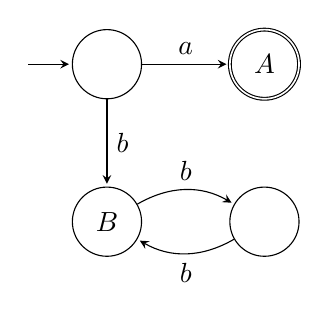
\begin{tikzpicture}[%
    >=stealth,
	shorten >=1pt,
	node distance=2cm,
%    on grid,
    auto,
%    state/.append style={minimum size=2em},
%    thick
  ]
    \node[state] (S)              {};
    \node[state,double] (A) [right of=S] {$A$};
    \node[state] (B) [below of=S] {$B$};
    \node[state] (C) [right of=B] {};

    \path[->] (S) +(-1,0) edge (S)
              (S)         edge              node {$a$} (A)
              (S)         edge              node {$b$} (B)
              (B)         edge  [bend left]            node {$b$} (C)
              (C)         edge  [bend left]            node {$b$} (B)
              ;
  \end{tikzpicture}
  
This is a deterministic automaton for the language $\Set{a} \in \Lang^*(\mathrm{FO[<]})$. If you make $B$ also a final state, we get the language $a + b(bb)^* \not\in \Lang^*(\mathrm{FO[<]})$.

So, E4 seems too restricted.

%S303.1: TODO: weniger ...

\end{itemize}

%\section{$* \rightarrow \omega$}

\subsection{Language Operators: Transformation of $*$-languages to $\omega$-languages}

We already introduced $\lim$ in \cref{reg:omega:vialangop}. We can define a family of language operators, partly also derived from the study of $\LangOreg$. Some of these operators operate on a single language and not on the class. Let $\Lang$ be a $*$-language class. Let $L \in \Lang$.

We define the following operators on languages, i.e. $\Power(\Sigma^*) \rightarrow \Power(\Sigma^\omega)$:
\begin{enumerate}
\item $\ext(L) := \Set{\alpha \in \Sigma^\omega}{ \exists n \colon \alpha[0,n] \in L} = L \cdot \Sigma^\omega$
\item $\dext(L) := \Set{\alpha \in \Sigma^\omega}{ \forall n \colon \alpha[0,n] \in L}$ (also called the dual-ext)
\item $\lim(L) := \Set{ \alpha \in \Sigma^\omega }{ \forall N \colon \exists n > N \colon \alpha[0,n] \in L } = \Set{ \alpha \in \Sigma^\omega }{ \exists^\omega n \colon \alpha[0,n] \in L }$
\item $\dlim(L) := \Set{ \alpha \in \Sigma^\omega }{ \exists N \colon \forall n > N \colon \alpha[0,n] \in L }$ (also called dual-lim)
\end{enumerate}

From these, we get operators on language classes ($\Power(\Power(\Sigma^*)) \rightarrow \Power(\Power(\Sigma^\omega))$) in a canonical way:
\begin{enumerate}
\item $\ext(\Lang) := \Set{\lim L}{L \in \Lang}$
\item $\dext(\Lang) := \Set{\dext L}{L \in \Lang}$
\item $\lim(\Lang) := \Set{\lim L}{L \in \Lang}$
\item $\dlim(\Lang) := \Set{\dlim L}{L \in \Lang}$
\end{enumerate}

Note that we sometimes combine those operators via union or intersection, e.g. $\ext \cup \dext \Lang := \ext \Lang \cup \dext \Lang$ or $\ext \cup \lim \Lang := \ext \Lang \cup \lim \Lang$. In many cases, it is also interesting to look at boolean combinations of $\omega$-language classes, i.e.:
\begin{enumerate}
\item $\BC \ext \Lang = \BC (\ext (\Lang))$
\item $\BC \lim \Lang = \BC (\lim (\Lang))$
\end{enumerate}

In addition, from historical reasons (compare with the definition and alternative characterizations of $\LangOreg$ in \cref{reg-omega-lang}), we also have the following other language class operators:
\begin{enumerate}
\item $\displaystyle \Kleene(\Lang) := \Set{ \bigcup_{i=1}^n U_i \cdot V_i^\omega}{U_i, V_i \subseteq \Sigma^*, U_i \cdot V_i^* \in \Lang, n \in \N_0}$
\item $\displaystyle \limClosure(\Lang) := \Set{\bigcup_{i=1}^n U_i \cdot \lim V_i}{U_i, V_i \subseteq \Sigma^*, U_i \cdot V_i^* \in \Lang, n \in \N_0}$
\end{enumerate}
In \cref{reg-omega-lang}, we have seen that
\[ \BC \lim \Langreg = \Kleene \Langreg = \limClosure \Langreg . \]

We mostly concentrate on $\ext$, $\lim$ and boolean combinations of them in the rest of this thesis.

For $\ext$ and $\dext$, we can also introduce equivalent $\omega$ automata acceptance conditions (as in \cite{InfCompR101}). Let $L \subseteq \Sigma^*$ be a regular $*$-language and $\A = (Q, \Sigma, q_0, \Delta, F)$ be an automaton which accepts exactly $L$. Let $\alpha \in \Sigma^\omega$. Then
\begin{itemize}
\item $\A$ \defword{E-accepts} $\alpha \ \ \ :\Leftrightarrow \ \ \ \exists \ \text{infinite run $\rho$ in $\A$ which matches $\alpha$} \colon \exists i \colon \rho[i] \in F$,
\item $\A$ \defword{A-accepts} $\alpha \ \ \ :\Leftrightarrow \ \ \ \exists \ \text{infinite run $\rho$ in $\A$ which matches $\alpha$} \colon \forall i \colon \rho[i] \in F$.
\end{itemize}
We define
\begin{itemize}
\item[] $L^\omega_E(\A) := \Set{\alpha \in \Sigma^\omega}{\text{$\alpha$ is E-accepted in $\A$}}$,
\item[] $L^\omega_A(\A) := \Set{\alpha \in \Sigma^\omega}{\text{$\alpha$ is A-accepted in $\A$}}$,
\end{itemize}
and we have the equalities
\begin{itemize}
\item[] $L^\omega_E(\A) = \ext(L)$,
\item[] $L^\omega_A(\A) = \dext(L)$.
\end{itemize}
Note that $\A$ can be both deterministic or non-deterministic for this property (see \cref{gen:e-determinism}).

In a similar way, the $\lim$ operator is equivalent to the Büchi acceptance condition on deterministic automata. Here the determinism matters --- non-deterministic Büchi automata are strictly more powerful. For the $\dlim$ operator, we can also introduce an equivalent automata acceptance condition: An automaton $\A = (Q,\Sigma,q_0,\Delta,F)$ \defword{co-Büchi-accepts} an infinite word $\alpha \in \Sigma^\omega$ iff there is a matching infinite run $\rho \in Q^\omega$ such that $\exists N \colon \forall n \ge N \colon \rho[n] \in F$.

The relations between the E-acceptance / the $\ext$ operator or the A-acceptance / the $\dext$ operator with Büchi / $\lim$ or co-Büchi / $\dlim$ are inspired historically from \cite{Landweber69}. Landweber originally introduced the 1,1',2,2',3-acceptance conditions which are equivalent to the E,A,Büchi,co-Büchi and Muller acceptance conditions.

\

Given these language operators, we are interested in the relations between them. For the class $\Langreg$ of regular languages, we already know that
\[ \LangOreg = \Kleene(\Langreg) = \BC \lim (\Langreg) = \limClosure(\Langreg) . \]

\subsection{Classification of regular $\omega$-languages} %$\Langreg$

\label{regomega-diagram}
Considering $\mathcal{R} := \Langreg$, we get the following language diagram:

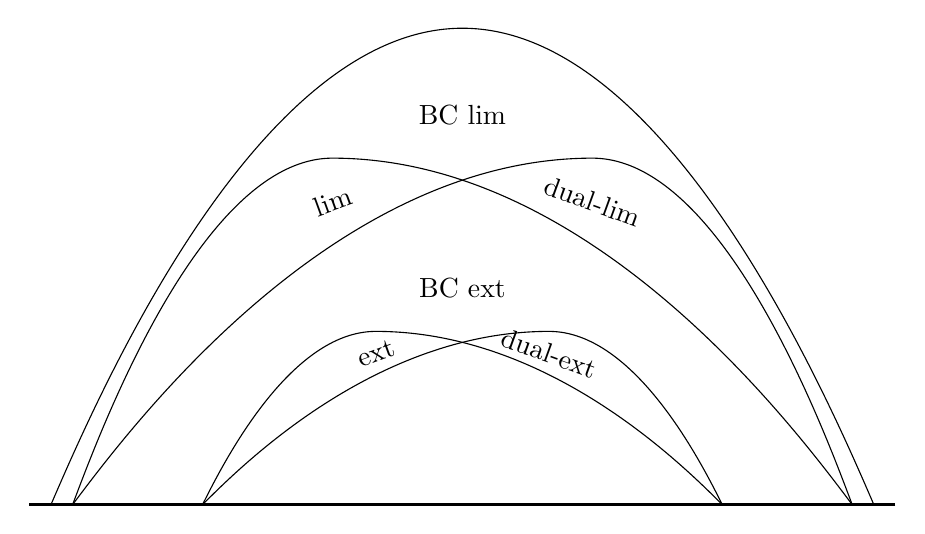
\begin{tikzpicture}
\pgftransformscale{.55}

% http://www.texample.net/tikz/examples/complexity-classes/

%%% HELP LINES - uncomment to design/extend
% \draw[step=1cm,gray,very thin] (-10,0) grid (10,12);
% \node at (0,0) {\textbf{(0,0)}};

%% Horizontal bar
\draw[very thick] (10,0) -- (-10,0);

% BC lim
\draw (-9.5,0) parabola bend (0,11) (9.5,0);
\node at (0,9) {BC lim};

% lim
\draw (-9,0) parabola bend (-3,8) (9,0);
\node[rotate=20] at (-3,7) {lim};

% dual-lim
\draw (-9,0) parabola bend (3,8) (9,0);
\node[rotate=-20] at (3,7) {dual-lim};

% BC ext
%\draw (-6.5,0) parabola bend (0,6) (6.5,0);
\node at (0,5) {BC ext};

% ext
\draw (-6,0) parabola bend (-2,4) (6,0);
\node[rotate=20] at (-2,3.5) {ext};

% dual-ext
\draw (-6,0) parabola bend (2,4) (6,0);
\node[rotate=-20] at (2,3.5) {dual-ext};

\end{tikzpicture}

where all inclusions are strict. This is basically Landweber's Theorem from \cite{Landweber69}. In more detail and a bit extended from Landweber's Theorem:

% overview of references: S50.1
% S50.2:
\begin{theorem}[Landweber]
\label{P:reg-star}

\begin{enumerate}
\item[1.] $\ext \mathcal{R} \cap \dext \mathcal{R} \neq \emptyset$
\item[2a.] $\ext \mathcal{R} \cap \dext \mathcal{R} \subsetneqq \ext \mathcal{R}$
\item[2b.] $\ext \mathcal{R} \cap \dext \mathcal{R} \subsetneqq \dext \mathcal{R}$
\item[3.] $\ext \mathcal{R} \neq \dext \mathcal{R}$
\item[4.] $\ext \mathcal{R} \cup \dext \mathcal{R} \subsetneqq \BC \ext \mathcal{R}$
\item[5.] $\BC \ext \mathcal{R} = \lim \mathcal{R} \cap \dlim \mathcal{R}$ (Staiger-Wagner class)
\item[6a.] $\lim \mathcal{R} \cap \dlim \mathcal{R} \subsetneqq \lim \mathcal{R}$
\item[6b.] $\lim \mathcal{R} \cap \dlim \mathcal{R} \subsetneqq \dlim \mathcal{R}$
\item[7.] $\lim \mathcal{R} \neq \dlim \mathcal{R}$
\item[8.] $\lim \mathcal{R} \cup \dlim \mathcal{R} \subsetneqq \BC \lim \mathcal{R}$
\end{enumerate}
and we have the additional equalities
\begin{enumerate}
\item[9.] $\BC \lim \mathcal{R} = \Kleene(\mathcal{R})$
\item[10.] $\BC \lim \mathcal{R} = \limClosure(\mathcal{R})$
\item[11.] $\BC \lim \mathcal{R} = \Set{L_{\text{Büchi}}^\omega(\A)}{\A \text{ non-det. automaton so that } L^*(\A) \in \mathcal{R}}$
\end{enumerate}

\begin{proof}
\begin{enumerate}
\item[1.] $\tilde{L}_1 := a \Sigma^\omega \in \ext \cap \dext \mathcal{R}$ with $\tilde{L}_1 = \ext(a)$ and $\tilde{L}_1 = \dext (\Set{\epsilon} \cup a \Sigma^*)$. (\cite[prop, p.38]{InfCompR101})
\item[2a.] $\tilde{L}_{2a} := \ext(a^* b) = a^* b \Sigma^\omega \in \ext \mathcal{R}$. Assume some A-automaton $\A$ with $n$ states accepts $\tilde{L}_{2a}$. $\A$ would also accept $a^n b^\omega$. I.e. the $(n+1)$th state after the run of $a^n$ would also accept $a$, i.e. $\A$ would accept $a^{n+1}$. By inclusion, $\A$ would accept $a^\omega$. That is a contradiction. Thus, there is no such A-automat. Thus, $\tilde{L}_{2a} \notin \dext \mathcal{R}$.
\item[2b.] $\tilde{L}_{2b} := - \tilde{L}_{2a} \in \dext \mathcal{R}$, $\tilde{L}_{2b} \notin \ext \mathcal{R}$.
\item[3.] Follows directly from P2a and P2b.
\item[4.] $\tilde{L}_4 := \Sigma^* a \Sigma^\omega \cap -(\Sigma^* b \Sigma^\omega)$, $\Sigma = \Set{a,b,c}$. Then we have $\tilde{L}_4 \notin \ext \cup \dext \mathcal{R}$, $\tilde{L}_4 \in \BC \ext \mathcal{R}$. (\cite[p.38]{InfCompR101})

\item[5.]
%S405 / Staigner-Wagner-recognizable
A language in this class is also said to have the \defword{obligation property}. Staiger and Wagner have introduced a \defword{Staiger-Wagner automaton} (also called a \defword{weak Muller automaton}; see definition \ref{def:staiger-wagner}) which can accept exactly this language class. This class of languages is called the \defword{Staiger-Wagner-recognizable} languages. This is stated in \cref{thm:staiger-wagner}.

%Given an automaton $\A = (Q,\Sigma,q_0,\Delta,\F)$ with $\F \subseteq 2^Q$, a run $\rho$ in $\A$ is \defword{Staiger-Wagner-accepted} iff $\Occ(\rho) \in \F$, where $\Occ(\rho) := \Set{q \in Q}{\text{$q$ occurs in $\rho$}}$.

A generic proof of the equality $\BC \ext \mathcal{R} = \lim \mathcal{R} \cap \dlim \mathcal{R}$ is given in \cref{gen:staiger-wagner}.

\item[6a.] $\tilde{L}_{6a} := \lim(\Sigma^* a) = (\Sigma^* a)^\omega$. Assume there is $L \subseteq \Sigma^*$ with $\lim(L) = -\tilde{L}_{6a}$. Let $(w_0,w_1,w_2,\dotsc) \in (\Sigma^*)^\N$ so that $w_0 \in L, w_0 a w_1 \in L, \dotsc, w_0 \prod_{i=0}^n a w_i \in L \ \forall n \in \N$. Thus, $\alpha := w_0 \prod_{i \in \N} a w_i \in \lim L$. But $\alpha \notin -\tilde{L}_{6a}$. That is a contradiction. Thus, $-\tilde{L}_{6a} \notin \lim \mathcal{R}$. Because $\mathcal{R}$ is closed under complement, we get $\tilde{L}_{6a} \notin \dlim \mathcal{R}$.
\item[6b.] Analog to 6a with $\tilde{L}_{6b} := -\tilde{L}_{6a}$.
\item[7.] Follows directly from 6a and 6b.

\item[8.]
%(S408, S409)
$\tilde{L}_8 := (\Sigma^*a)^\omega \cap -(\Sigma^*b)^\omega$. Then $\tilde{L}_8 \notin \lim \cup \dlim \mathcal{R}$ but $\tilde{L}_8 \in \BC \lim \mathcal{R}$. (\cite[prop, p.38]{InfCompR101})

\item[9.-11.]
%(S402, S407)
%(S403, S411) (R107, Theorem 3.1)
This is explained already in \cref{reg-omega-lang} and in more detail in \cite{InfCompR101} or \cite[Theorem 3.1]{CombR107}.

\end{enumerate}
\end{proof}
\end{theorem}

%\subsection{Towards a theory for subclasses of the regular language class} %Questions

This relation diagram was studied in detail for $\Langreg$ and the main relations where shown by Landweber in \cite{Landweber69}. In addition to the strict inclusions of the expressiveness power of the different automata acceptance conditions, he also showed that it is decideable for a Muller automaton to tell wether its accepted language can also be accepted by an E-/A-/Büchi-/co-Büchi-automaton, respectively.

We are interested wether we get the same properties for other $*$-language classes under the given language operators.

% \stackrel{?}{\le} or \overset{?}{\le}
%Esp.:
%\begin{itemize}
%\item $\BC \ext \Lang \overset{?}{\subsetneqq} \BC \lim \Lang$
%\end{itemize}

In \cref{general-results}, we will reformulate many proofs of the properties given in \cref{P:reg-star} in a generic way. The results will give us an understanding about when such $\omega$-language class relations hold, when inclusions are strict and when they are not.

These base theorems are then used in \cref{concrete-results} to study some concrete $*$-language classes.

%% Quelle: Automata, Semigroups, Logic and Games - Pin, Perrin

\section{Automat}

Ein \defword{Automat} $\A$ auf dem Alphabet $\Sigma$ ist gegeben durch eine Menge $Q$ von Zuständen und einer Teilmenge $E \subset Q \times A \times Q$ von Transitionen. Außerdem ist in der Regel eine Teilmenge $I \subset Q$ von Startzuständen und eine Teilmenge $F \subset Q$ von Endzuständen gegeben.

Wir schreiben dafür: $\A = (Q, \Sigma, E, I, F)$.

Der Automat ist endlich genau dann, wenn $Q$ und $\Sigma$ endlich sind.

Der Automat ist deterministisch, wenn $E$ eine Menge von Funktionen $Q \times A \rightarrow \Q$ und wenn $|I| = 1$ sind.

\subsection{Pfad}
Zwei Transitionen $(p,a,q), (p',a',q') \in E$ sind aufeinanderfolgend, wenn $q=p'$.

Ein Pfad in dem Automat $\A$ ist eine Folge von aufeinanderfolgenden Transitionen, geschrieben als:
$q_0 \rightarrow^{a_0} q_1 \rightarrow^{a_1} q_2 \dots$

\subsection{Akzeptanz von endlichen Wörtern}

Ein Automat $\A = (Q, \Sigma, E, I, F)$ \defword{akzeptiert} ein endliches Wort $w = (a_0,a_1,...,a_n) \in \Sigma^*$ genau dann, wenn es einen Pfad $q_0 \rightarrow^{a_0} q_1 \rightarrow^{a_1} q_2 \dots \rightarrow^{a_n} q_{n+1}$ gibt mit $q_0 \in I$ und $q_{n+1} \in F$.

Die Sprache $L^*(\A)$ ist definiert als die Menge aller Wörter, die von $\A$ akzeptiert werden.

\section{$*$-Sprachklassen}
Die $*$-Sprachklasse ist die Menge aller Sprachen von Wörtern $w \in \Sigma^*$, also die Menge von Sprachen von endlichen Wörtern.

\subsection{reguläre Sprachen}
Eine Sprache ist genau dann regulär, wenn sie von einem endlichen Automat erkannt wird.

\subsection{piece-wise testable}


\subsection{$k$-locally testable}


\subsection{dot-depth-$n$}
\subsection{starfree}
\subsection{locally modulo testable}
\subsection{$R$-trivial}
\subsection{endlich / co-endlich}
\subsection{endwise testable}

\section{$\omega$-Sprachklassen}
\subsection{Büchi Automat}
Ein Automat $\A = (Q, \Sigma, E, I, F)$ \defword{Büchi-akzeptiert} ein Wort $w = (a_0,a_1,a_2,...) \in \Sigma^\omega$ genau dann, wenn es einen unendlichen Pfad $q_0 \rightarrow^{a_0} q_1 \rightarrow^{a_1} q_2 \rightarrow^{a_2} q_3 ...$ gibt mit $q_0 \in I$ und $\{ q_i | q_i \in F \}$ unendlich, also der unendlich oft einen Zustand $F$ erreicht.

Die Sprache $L^\omega(\A)$ ist definiert als die Menge aller unendlichen Wörter, die von $\A$ Büchi-akzeptiert werden.

Man bezeichnet einen Automaten $\A$ als Büchi Automat, wenn man von der Büchi-Akzeptanz ausgeht.

\subsection{Muller Automat}
Ein Muller Automat $\A$ ist ein endlicher, deterministischer Automat mit Muller Akzeptanzbedingung und einer Menge $\T \in 2^Q$, genannt die Tabelle des Automaten (anstatt der Menge $F$). Dabei wird ein Wort $w \in \Sigma^\omega$ akzeptiert genau dann, wenn es einen entsprechenden Pfad $p$ gibt mit $\Inf(p) \in \T$, wobei $\Inf(p)$ die Menge der unendlich oft besuchten Zustände ist.

Wir schreiben $\A = (Q, \Sigma, E, i, \T)$.

\subsection{Rabin Automat}
Ein Rabin Automat ist ein Tuple $\A = (Q, \Sigma, E, i, \R)$, wobei $(Q,\Sigma,E)$ ein deterministischer Automat ist, $i$ ist der Startzustand und $\R = \{(L_j, U_j) | j \in J\}$ ist eine Familie von Paren von Zustandsmengen. Ein Pfad $p$ ist erfolgreich, wenn er in $i$ beginnt und wenn es einen Index $j \ in J$ gibt, so dass $p$ unendlich oft $U_j$ besucht und nur endlich oft $L_j$. Ist der Automat endlich, so ist dies äquivalent mit
\[ \Inf(p) \cap L_j = \emptyset \ \text{und} \ \Inf(p) \cap U_j \neq \emptyset . \]

\subsection{Staiger Wagner Klasse zu $\K$}

\section{Operationen: von $*$-Sprache $K$ zu $\omega$-Sprache $L_\omega (K)$}
\subsection{...}
a)
* alle Sprachen $K \dot \Sigma^\omega = \ext(K)$, $K \in \K$

* offene G

* Staiger Wagner Klasse
http://de.wikipedia.org/wiki/Staiger-Wagner-Automat
Erich Grädel, Wolfgang Thomas und Thomas Wilke (Herausgeber), Automata, Logics, and Infinite Games, LNCS 2500, 2002, Seite 20 (auf englisch)
http://www.automata.rwth-aachen.de/material/skripte/areas-english.pdf - s.53

a')
dual $\overline{K}$ = $\omega$-Wörter, deren alle Präfixe in $K$ sind

b) Sprachen $\lim \K$
BC Muller-erkennbare
(BC: boolean closure ?)

b') von einer Stelle an alle Prefixe in $K$

c) Kleene-Closure

alle der Form $\cup_{i=1}^n U_i \dot V_i^\omega$, $U_i, V_i \in \K$

d) $\K$ nicht suffix sensitiv

$K \in \K \Rightarrow K \dot \Sigma^* \in \K$  

\section{General results}
\label{general-results}

%S401, S303: TODO

Let $\Lang$ be a $*$-language class.

\subsection{general}
Let $L \in \Lang$.
\begin{itemize}
\item $\ext L = L \cdot \Sigma^\omega$
\item $\ext L = \lim (L \cdot \Sigma^*)$
\item $- \lim(-L) = \dlim L$
\end{itemize}

\

%S302.1:
We are interested in relations like $\BC \ext \Lang \overset{?}{\subsetneqq} \BC \lim \Lang$ or $\ext \Lang \overset{?}{\subsetneqq} \lim \Lang$. With $\Lang = \Set{\Set{a}}$, we realize that even $\ext \Lang \subseteq \lim \Lang$ is not true in general ($\ext \Set{\Set{a}} = \Set{a \Sigma^\omega} \neq \emptyset = \lim \Set{\Set{a}}$). In \ref{gen:non-suffix-sens}, we see a sufficient condition for this property, though.

\subsection{$\ext \subset \lim$}
\label{gen:S302a}

%S302:
From $\ext \Lang \subseteq \lim \Lang$, it directly follows $\Set{-\ext L}{L \in \Lang} \subseteq \Set{-\lim L}{L \in \Lang}$. Thus, it also follows $\BC \ext \Lang \subseteq \BC \lim \Lang$.

\subsection{$\dext \subset \dlim$}

%S302:
From $\ext \Lang \subseteq \lim \Lang$, we need E3 ($\Lang$ closed under negation) to get $\dext \Lang \subseteq \dlim \Lang$. This is in contrast to \ref{gen:S302a}, where it directly follows. We have to be careful about the difference $- \ext \Lang \neq \dext \Lang$. 

\subsection{non suffix sensitive}
\label{gen:non-suffix-sens}

% S303, S101a:
E1 ($\forall L \in \Lang \colon L \cdot \Sigma^* \in \Lang$)
$\Rightarrow \ext(\Lang) \subseteq \lim(\Lang)$

\subsection{union, intersection}
%S303:
\begin{itemize}
\item
E2a (closed under union) $\Rightarrow \bigcup \ext \Lang \subseteq \ext \Lang$.
\item
E2b (closed under intersection) $\Rightarrow \bigcap \ext \Lang \subseteq \ext \Lang$.
\end{itemize}

\subsection{$op \cup \overline{op} \subsetneqq \BC op$}
If there is $L_\Sigma \in \Lang_\Sigma$ with $L_\Sigma \in \ext \Lang_\Sigma, L_\Sigma \not\in \dext \Lang_\Sigma$ and E3 (closed under negation) holds for $\Lang$:
\begin{itemize}
\item[$\Rightarrow$] $-L_\Sigma \in \dext \Lang_\Sigma, -L_\Sigma \not\in \ext \Lang_\Sigma$
\item[$\Rightarrow$] $L_{\Sigma_1} \cup -L_{\Sigma_2} \in \BC \ext \Lang_{\Sigma_1 \dot{\cup} \Sigma_2}$ \newline
$L_{\Sigma_1} \cup -L_{\Sigma_2} \not\in \ext \cup \dext \Lang_{\Sigma_1 \dot{\cup} \Sigma_2}$
\end{itemize}
Thus, $\ext \cup \dext \Lang \subsetneqq \BC \ext \Lang$.

Similarily, if there is $L_\Sigma \in \lim \Lang_\Sigma, L_\Sigma \not\in \dlim \Lang_\Sigma$ and E3 holds for $\Lang$:
\begin{itemize}
\item[$\Rightarrow$] $-L_\Sigma \in \dlim \Lang_\Sigma, -L_\Sigma \not\in \lim \Lang_\Sigma$
\item[$\Rightarrow$] $L_{\Sigma_1} \cup -L_{\Sigma_2} \in \BC \lim \Lang_{\Sigma_1 \dot{\cup} \Sigma_2}$ \newline
$L_{\Sigma_1} \cup -L_{\Sigma_2} \not\in \lim \cup \dlim \Lang_{\Sigma_1 \dot{\cup} \Sigma_2}$
\end{itemize}
Thus, $\lim \cup \dlim \Lang \subsetneqq \BC \lim \Lang$.


\subsection{$\BC \lim = \lim \cap \dlim$}
\label{gen:staigner-wagner}
%S402: TODO...
%S405:
Staigner-Wagner-recognizable
%S305:

\subsection{Kleene-star $= \BC \lim$}
\label{gen:kleene-star}
%S407

%S306:

\section{Results on concrete $*$-language classes}
\label{concrete-results}

%\subsection{Overview}
%...
In \cref{chapter:regOmegaLangs}, we already showed many results for the different $\omega$-language classes constructed based on $\Langreg$. Mainly, those are the strict inclusions as shown in the diagram in \cref{regomega-diagram}.

In \cref{general-results}, we found some general conditions on abritrary $*$-language classes $\Lang$ under which the inclusion diagram stays the same. We also gave other conditions on $\Lang$ under which the diagram becomes different or other properties change.

We will now study some concrete well-known $*$-language classes and try to apply the results from \cref{general-results} as well as study some properties individually.

%S15/S151: overview, hierarchy

\subsection{Starfree regular languages}
%S18: def
The set of \defword{star-free $*$-languages} $\Lang(\mathtext{starfree})$ is defined as the smallest set $\Lang = \Lang(\mathtext{starfree})$ with
\begin{itemize}
\item[(a)] $\Set{a} \in \Lang$ for all $a \in \Sigma$,
\item[(b)] $\Lang$ is closed under boolean operations,
\item[(c)] $\Lang$ is closed under concatenation.
\end{itemize}
See \cite[Section 2.2]{ConcHierR104} for further references.

This class is also equivalent to the set of $\mathrm{FO[<]}$-definable languages. %TODO: ref
%W161,S210,S211,S101a,S51
% R107: some characterization
%In \cite[Theorem 3.2]{CombR107}, we see that
%\[  \Lang^\omega(\Set{}) ... \]

First, we start with some specific study on this language class.

%S210:
\begin{theorem}
\[ \Lang^\omega (\mathrm{FO[<]}) = \BC \lim \Lang^*(\mathrm{FO[<]}) \]
\begin{proof}
Let $\varphi \in \mathrm{FO[<]}$. By the \cite[Normal Form Theorem (4.4)]{CombR107} there are bounded formulas $\varphi_1(y),\dotsb,\varphi_r(y),\psi_1(y),\dotsb,\psi_r(y)$ such that for all $\alpha \in \Sigma^\omega$:
\[ \alpha \models \varphi \Leftrightarrow \alpha \models \bigvee_{i=1}^r \left( \forall x \exists y > x \colon \varphi_i (y) \right) \wedge \neg \left( \forall x \exists y > x \colon \psi_i (y) \right) \]
Thus:
\[
\alpha \models \varphi \Leftrightarrow \bigvee_{i=1}^r
\underbrace{ \left( \alpha \models \forall x \exists y > x \colon \varphi_i (y) \right) }_
{\mathclap{\quad\quad \begin{aligned}
& \Leftrightarrow \forall x \exists y > x \colon \alpha[0,n] \models \varphi_i(\omega) \\
& \Leftrightarrow \exists^\omega n \colon \alpha[0,n] \models \varphi_i(\omega) \\
& \Leftrightarrow \alpha \in \lim L^*( \varphi_i(\omega) )
\end{aligned}}}
\wedge \neg \left( \alpha \models \forall x \exists y > x \colon \psi_i (y) \right)
\]
where $\varphi_i(\omega)$ stands for $\varphi_i$ with all bounds removed.
I.e. we have
\[ L^\omega(\varphi) = \bigcup_{i=1}^r \lim( L^* (\varphi_i (\omega)) \cap \neg \lim( L^* (\psi_i (\omega))) , \]
and thus
\[ L^\omega(\varphi) \in \BC \lim \Lang^* (\mathrm{FO[<]}) . \]
We have prooved the $\subseteq$-direction. For $\supseteq$:
\begin{align*}
& \alpha \in \lim( L^*(\varphi) ) \\
\Leftrightarrow \ & \exists^\omega n \colon \alpha[0,n] \models \varphi \\
\Leftrightarrow \ & \alpha \models \forall x \exists y > x \colon \varphi(y) \\
\Leftrightarrow \ & \alpha \in L^\omega ( \forall \exists y > x \colon \varphi(y) )
\end{align*}
where $\varphi(y)$ stands for $\varphi$ with all variables bounded by $y$.
I.e.
\[ \lim \Lang^* (\mathrm{FO[<]}) \subseteq \Lang^\omega (\mathrm{FO[<]}) , \]
and thus also
\[ \BC \lim \Lang^* (\mathrm{FO[<]}) \subseteq \Lang^\omega (\mathrm{FO[<]}) . \]
Thus we have prooved the equality.
\end{proof}
\end{theorem}

%S211:
\begin{theorem}
\[ \BC \ext \Lang^*( \mathrm{FO[<]} ) \subsetneqq \BC \lim \Lang^* ( \mathrm{FO[<]} ) \]
\begin{proof}
$\subseteq$: $L \subset \Sigma^\omega \text{ starfree } \ \Rightarrow\ L \Sigma^\omega \in \lim( \Lang^*( \mathrm{FO[<]} ) )$

$\neq$:
\begin{align*}
& L := (\Sigma^* a)^\omega \\
\Rightarrow \ & L = \lim( (\Sigma^* a)^* ) \\
\Rightarrow \ & L = L^\omega(\exists^\omega x : Q_a x)
\end{align*}
And we have $L \notin \BC \ext \Lang^* (\mathrm{FO[<]})$.
\end{proof}
\end{theorem}

%S101a:
$\Set{a} \in \Lang$. $a \Sigma^* \in \Lang$, thus $a\Sigma^\omega = \ext(\Set{a}) = \dext{a\Sigma^*}$. I.e. $\ext \cap \dext \Lang \ne \emptyset$.

$\Lang^*( \mathrm{FO[<]} )$ is obviously \emph{closed under negation, suffix-independence, union and alphabet permutation}.

We can also see that $\Lang^*( \mathrm{FO[<]} )$ is \emph{closed under change of final states}. %TODO: argue

$L_a := \Sigma^* a \in \Lang$ is a $\ext$-$\dext$-separating and $\lim$-$\dlim$-separating language.

Thus, with \cref{gen:main-theorem-inclusions}, we get
\[ \ext \cap \dext \Lang \subsetneqq
\ext \cup \dext \Lang \subsetneqq
\BC \ext \Lang =
\lim \cap \dlim \Lang \subsetneqq
\lim \cup \dlim \Lang \subsetneqq
\BC \lim \Lang . \]


\subsection{Piecewise testable languages}
%S19: def
\label{lang:PT}
Let $u,v \in \Sigma^*$. For $n \in \N$, define the congruence relation $\simeq_{\PT_n}$:
\[ u \simeq_{\PT_n} v \ \ \ :\Leftrightarrow \ \ \ \operatorname{Subwords}_{\le n}(u) = \operatorname{Subwords}_{\le n}(v) , \]
where
\[ \operatorname{Subwords}_{\le n}(u) := \Set{w \in \Sigma^{\le n}}{\text{$w$ is a subword of $u$}} \]
and $w$ is a \defword{subword} of $u$ for $w,u \in \Sigma^*$ iff there is a subsequence $(s_n)_{n\in\N}$ of $(n)_{n\in\N}$ such that $w = u|_s$.

Define
\[ \Lang(\PT_n) := \Lang(\simeq_{\PT_n}). \]
Then the class of \defword{piecewise testable languages} is defined as
\[ \Lang(\PT) := \bigcup_{n\in\N} \Lang(\PT) . \]

We also have the characterization
\[ \Lang(\PT) = \BC \bigcup_{n\in\N_0,a_i \in \Sigma} \Set{\Sigma^* a_1 \Sigma^* a_2 \Sigma^* \cdots\Sigma^* a_n \Sigma^*} . \]
% The syntactic monoid is also J-trivial.

See \cite[Section 2.3]{ConcHierR104} for further references.

%S52: overview
%S212: BC lim class

$L$ piece-wise testable $\Leftrightarrow$ $L$ is a boolean algebra of $\Sigma^* a_1 \Sigma^* a_2 \dotsb a_n \Sigma^*$.

%S101:
\begin{theorem}
\label{thm.PT}
\[ \BC \ext \Lang^* (\PT) = \BC \lim \Lang^* (\PT) \]
\begin{proof}
$\subseteq$: It is sufficient to show $\ext(\Lang^* (\PT)) \subseteq \BC \lim \Lang^* (\PT)$.

By complete induction:
\begin{align*}
& \ext(\Sigma^* a_1 \Sigma^* a_2 \dotsb a_n \Sigma^*) = \Sigma^* a_1 \Sigma^* a_2 \dotsb a_n \Sigma^\omega = \lim(\Sigma^* a_1 \Sigma^* a_2 \dotsb a_n \Sigma^*) \\
& \ext( \neg ( \Sigma^* a_1 \Sigma^* a_2 \dotsb a_n \Sigma^* )) = \Sigma^\omega = \lim( \Sigma^* ) \\
& \ext( \emptyset ) = \emptyset = \lim(\emptyset)
\end{align*}

It is sufficient to show negation only for such ground terms because we can always push the negation down.
\begin{align*}
& \ext(A \cup B) = \ext(A) \cup \ext(B) \\
& \ext(A \cap B) = \ext(A) \cap \ext(B)
\end{align*}

This makes the induction complete.

$\supseteq$: It is sufficient to show $\lim(\Lang^* (\PT)) \subseteq \BC \ext \Lang^* (\PT)$.
\begin{align*}
& \lim(\emptyset) = \ext(\emptyset), \ \lim(\Sigma^* a_1 \Sigma^* a_2 \dotsb a_n \Sigma^*) = \ext(\Sigma^* a_1 \Sigma^* a_2 \dotsb a_n \Sigma^*) \ \ \text{(see above)} \\
& \begin{aligned}
\lim( \neg ( \Sigma^* a_1 \Sigma^* a_2 \dotsb a_n \Sigma^* ) ) & = \Set{ \alpha \in \Sigma^\omega }{ \exists^\omega n \colon \alpha [0,n] \notin \Sigma^* a_1 \Sigma^* a_2 \dotsb a_n \Sigma^* } \\
& = \Set{ \alpha \in \Sigma^\omega }{ \forall n \colon \alpha [0,n] \notin \Sigma^* a_1 \Sigma^* a_2 \dotsb a_n \Sigma^* } \\
& = \neg \ext( \Sigma^* a_1 \Sigma^* a_2 \dotsb a_n \Sigma^* )
\end{aligned} \\
& \begin{aligned}
\lim(A \cup B) & = \Set{ \alpha \in \Sigma^\omega }{ \exists^\omega n \colon \alpha[0,n] \in A \cup B } = \lim(A) \cup \lim(B) \\
\lim(A \cap B) & = \Set{ \alpha \in \Sigma^\omega }{ \exists^\omega n \colon \alpha[0,n] \in A \cap B } \\
\intertext{and because $A,B$ are piece-wise testable}
& = \Set{ \alpha \in \Sigma^\omega }{ \exists n : \forall m > n \colon \alpha[0,m] \in A \cap B } = \lim(A) \cap \lim(B)
\end{aligned}
\end{align*}
\end{proof}
\end{theorem}



\label{lang:posPT}
\defword{Positive piece-wise testable languages} are defined as
\[ \Lang(\mathtext{pos-PT}) := \operatorname{pos-BC} \bigcup_{n\in\N_0,a_i \in \Sigma} \Set{\Sigma^* a_1 \Sigma^* a_2 \Sigma^* \cdots\Sigma^* a_n \Sigma^*} . \]

For positive piece-wise testable (pos-PT) languages, we get the same result.
%\subsection{positive piece-wise testable}
%S53: overview
%S214: BC lim class

%S101:
\begin{theorem}
\label{thm.ext.lim.posPT}
\[ \BC \ext \Lang^* (\mathtext{pos-PT}) = \BC \lim \Lang^* (\mathtext{pos-PT}) \]
\begin{proof}
$\subseteq$: Exactly like the proof for PT except that we leave out the negated part.

$\supseteq$: Also like the proof for PT.
\end{proof}
\end{theorem}

We also have a relation between pos-PT and PT.

\begin{theorem}
\[ \BC \ext \Lang^*(\mathtext{pos-PT}) = \BC \ext \Lang^* (\mathtext{PT}) \]

\begin{proof}
In the proof of $\lim \Lang^*(\mathtext{PT}) \subseteq \BC \ext \Lang^* (\mathtext{PT})$ we actually proved $\BC \lim \Lang^*(\mathtext{PT}) \subseteq \BC \ext \Lang^* (\mathtext{pos-PT})$. Similiarly we also proved $\BC \ext \Lang^* (\mathtext{PT}) \subseteq \BC \lim \Lang^* (\mathtext{pos-PT})$.

With \cref{thm.PT} and \cref{thm.ext.lim.posPT} we get the claimed equality.
\end{proof}
\end{theorem}


\subsection{Locally testable languages}
\label{lang:LT}
%S16: def
Let $u,v \in \Sigma^*$. For $n \in \N$, define the congruence relation $\simeq_{\text{LT}_n}$:
\begin{alignat*}{3}
u \simeq_{\text{LT}_n} v \ \ \ && :\Leftrightarrow \ \ \ & \operatorname{left-Fact}_{<n}(u) = \operatorname{left-Fact}_{<n}(v) , \\
&&& \operatorname{right-Fact}_{<n}(u) = \operatorname{right-Fact}_{<n}(v) , \\
&&& \operatorname{Fact}_{n}(u) = \operatorname{Fact}_{n}(v) \\
&& \Leftrightarrow \ \ \ & u \simeq_{\text{endwise}_n} v , \\
&&& \operatorname{Fact}_n(u) = \operatorname{Fact}_n(v)
\end{alignat*}
where
\begin{align*}
\operatorname{left-Fact}_{<n}(v) & := \Set{w \in \Sigma^{<n}}{\text{$w$ is left-factor of $v$}} \\
\operatorname{right-Fact}_{<n}(v) & := \Set{w \in \Sigma^{<n}}{\text{$w$ is right-factor of $v$}} \\
\operatorname{Fact}_{n}(v) & := \Set{w \in \Sigma^{n}}{\text{$w$ is factor of $v$}}.
\end{align*}
For $v,w \in \Sigma^*$,
\begin{align*}
\text{$w$ is a \defword{left-factor} of $v$} & \ :\Leftrightarrow \ \exists u \in \Sigma^* \colon wu = v \\
\text{$w$ is a \defword{right-factor} of $v$} & \ :\Leftrightarrow \ \exists u \in \Sigma^* \colon uw = v \\
\text{$w$ is a \defword{factor} of $v$} & \ :\Leftrightarrow \ \exists u_1,u_2 \in \Sigma^* \colon u_1 w u_2 = v.
\end{align*}

Define
\[ \Lang(\LT_n) := \Lang(\simeq_{\text{LT}_n}) . \]
Then the class of \defword{locally testable languages} is defined as
\[ \Lang(\LT) := \bigcup_{n\in\N} \Lang(\LT_n) . \]

We also have the characterization
\[ \Lang(\LT) = \BC \bigcup_{u,v,w \in \Sigma^+} \Set{u\Sigma^*, \Sigma^* v, \Sigma^* w \Sigma^*, \Set{\epsilon}} . \]

See \cite[Section 2.5]{ConcHierR104} for further references.

\begin{theorem}
\[ \BC \ext \Lang^* (\LT) \subsetneqq \BC \lim \Lang^*(\LT)  \]

\begin{proof}
Let $w \in \Sigma^+$.
\begin{align*}
& \ext (w \Sigma^*) = \lim(w \Sigma^*) \\
& \ext( \Sigma^* w) = \Sigma^* w \Sigma^\omega = \lim( \Sigma^* w \Sigma^* ) \\
& \ext( \Sigma^* w \Sigma^*) = \Sigma^* w \Sigma^\omega = \lim( \Sigma^* w \Sigma^* )
\end{align*}
Thus we have
\[ \BC \ext \Lang^* (\LT) \subseteq \BC \lim \Lang^*(\LT) . \]
But we also have
\[ \lim(\Sigma^*) = (\Sigma^* w)^\omega \notin \BC \ext \Lang^* (\LT) . \]
\end{proof}
\end{theorem}

% TODO: I think R105... handles them?
\defword{Positive locally testable languages} are defined as
\[ \Lang(\mathtext{pos-LT}) = \operatorname{pos-BC} \bigcup_{u,v,w \in \Sigma^+} \Set{u\Sigma^*, \Sigma^* v, \Sigma^* w \Sigma^*, \Set{\epsilon}} . \]

\subsection{Locally threshold testable languages}
\label{lang:LTT}
%S17: def
% FinAutLogR109
Let $u,v \in \Sigma^*$. Let $k,r \in \N$, define the congruence relation $\simeq_{\text{LTT}^k_r}$:
\begin{alignat*}{3}
u \simeq_{\text{LTT}^k_r} v \ \ \ && :\Leftrightarrow \ \ \ & \operatorname{left-Fact}_{<n}(u) = \operatorname{left-Fact}_{<n}(v) , \\
&&& \operatorname{right-Fact}_{<n}(u) = \operatorname{right-Fact}_{<n}(v) , \\
&&& \begin{aligned}
\forall x \in \Sigma^{\le k} \colon & \operatorname{count-Fact}_x(u) = \operatorname{count-Fact}_x(v) < r \ \ \ \ \text{or} \\
& \min \Set{\operatorname{count-Fact}_x(u), \operatorname{count-Fact}_x(v)} \ge r
\end{aligned}
\end{alignat*}
where for $x \in \Sigma^*$, $\operatorname{count-Fact}_x(u)$ states how often $x$ occurs as a factor in $u$, formally
\[ \operatorname{count-Fact}_x(u) := \#\Set{n \in \N}{u[n,n+\vert x \vert - 1] = x} . \]
Define
\[ \Lang(\text{LTT}^k_r) := \Lang(\simeq_{\text{LTT}^k_r}). \]
Then the class of \defword{locally threshold testable languages} is defined as
\[ \Lang(\mathtext{LTT}) := \bigcup_{k,r\in\N} \Lang(\text{LTT}^k_r) . \]

Locally threshold testable languages are a generalization of locally testable language. We can see that
\[  \Lang(\LT) = \bigcup_{k\in\N} \Lang(\text{LTT}^k_1) . \]

For further references, see \cite[IV.3]{FinAutLogR109}.

In \cite[IV.3.3]{FinAutLogR109}, we can see that
\[  \Lang(\text{LTT}) = \Lang(\mathrm{FO[+1]}). \]
%\subsection{FO[+1]}
%def: S17
%S213: BC ext class
%215: BC lim class

%S103:
\begin{theorem}
\[ \Lang^\omega (\mathrm{FO[+1]}) = \BC \ext \Lang^*(\mathrm{FO[+1]}) \]
\begin{proof}
From \cite[Theorem 4.8]{LangAutLogicR102}, we know that each formular in FO[+1] is equivalent (for both finite and infinite words) to a boolean combination of statements ``sphere $\sigma \in \Sigma^+$ occurs $\geq n$ times''. That statement can be expressed by a sentence of the form
\[ \psi := \exists \overline{x_1} \dotsb \exists \overline{x_n} \varphi(\overline{x_1}, \dotsb, \overline{x_n}) \]
where each $\overline{x_i}$ is a $\abs{\sigma}$-tuple of variables and the formula $\varphi$ states:
\[
\bigwedge_{\mathclap{i,j \in \underline{n},\atop { i \neq j,\atop k,l \in \underline{\abs{\sigma}}}}} x_{i,k} \neq x_{j,l}
\ \wedge\ \bigwedge_{\mathclap{i \in \underline{n},\atop k \in \underline{\abs{\sigma}-1}}} x_{i,k+1} = x_{i,k} + 1
\ \wedge\ \bigwedge_{\mathclap{i \in \underline{n},\atop k \in \underline{\abs{\sigma}}}} Q_{\sigma_k} x_{i,k}
\]
For $\psi$, we have:
\[ \alpha \models \psi \Leftrightarrow \exists n \colon \alpha[0,n] \models \psi \ \ \text{for all } \alpha \in \Sigma^\omega , \]
i.e.
\[ L^\omega(\psi) = \ext L^*(\psi) . \]
Any formular in FO[+1] can be expressed as a boolean combination of $\psi$-like formular. With
\begin{align*}
& L^\omega(\neg \psi) = \neg L^\omega(\psi) \\
& L^\omega(\psi_1 \wedge \psi_2) = L^\omega(\psi_1) \cap L^\omega(\psi_2) \\
& L^\omega(\psi_1 \vee \psi_2) = L^\omega(\psi_1) \cup L^\omega(\psi_2)
\end{align*}
we get:
\[ \Lang^\omega(\mathrm{FO[+1]}) = \BC \ext \Lang^*(\mathrm{FO[+1]}). \]
\end{proof}
\end{theorem}

\subsection{FO[]}

\subsection{Endwise testable languages}
\label{lang:endwise}
%S20: def
Let $u,v \in \Sigma^*$. For $n \in \N$, define the congruence relation $\simeq_{\text{endwise}_n}$:
\begin{alignat*}{3}
u \simeq_{\text{endwise}_n} v \ \ \ && :\Leftrightarrow \ \ \ & \operatorname{left-Fact}_{<n}(u) = \operatorname{left-Fact}_{<n}(v) , \\
&&& \operatorname{right-Fact}_{<n}(u) = \operatorname{right-Fact}_{<n}(v)
\end{alignat*}
Then the class of \defword{endwise testable languages} is defined as
\[ \Lang(\mathtext{endwise}) := \bigcup_{n\in\N} \Lang(\simeq_{\text{endwise}_n}) . \]

We also have the characterization
\[ \Lang(\mathtext{endwise}) = \Set{X \Sigma^* Y \cup Z}{X,Y \subseteq \Sigma^+, Z \subseteq \Sigma^*, \text{$X,Y,Z$ finite}} . \]

See \cite[Section 2.4]{ConcHierR104} for further references.

%S104:
\begin{itemize}
\item $\BC \ext \Lang^*(\mathtext{endwise}) \neq \BC \lim \Lang^*(\mathtext{endwise})$ because $\Sigma^*a \in \Lang^*(\mathtext{endwise})$.
\item $\ext(a\Sigma^* a) = a \Sigma^* a \Sigma^\omega \notin \BC \lim \Lang^*(\mathtext{endwise})$
\end{itemize}

\subsection{Local languages}
\label{lang:local}

\subsection{Finite / Co-finite languages}
\label{lang:finite}
%S105:
\begin{itemize}
\item $\lim \Lang^*(\mathtext{finite}) = \Set{\emptyset}$
\item $\ext \Lang^*(\mathtext{finite}) = \Lang^*(finite) \cdot \Sigma^\omega$
\item $\lim \Lang^*(\mathtext{co-finite}) = \Set{\Sigma^\omega}$
\item $\ext \Lang^*(\mathtext{co-finite}) = \Set{\Sigma^\omega}$
\end{itemize}

\subsection{Regular languages of dot-depth-$n$}
\label{lang:dotdepth}
%S21: def

\subsection{$L$-trivial languages}
\label{lang:Ltrivial}
\subsection{$R$-trivial languages}
\label{lang:Rtrivial}
%S23: def
\subsection{Locally modulo testable languages}
\label{lang:LmodT}
%S24: def

%\subsection{$k$-locally testable}

\subsection{Context free languages}
\label{lang:contextfree}



%!TEX root =  index.tex
\section{Conclusion}
\label{chapter:conclusion}

Via language class operators like $\ext$ or $\lim$, we induced $\omega$-language classes from $*$-language classes. We presented the known results on the relations of the induced $\omega$-language classes from $\Langreg$. Those relations were shown in the diagram in \cref{regomega-diagram}.

Then, we worked on several generic cases on arbitrary $*$-language classes $\Lang$ such that we get the expected inclusions as in the diagram or at least some of them. However, we have also seen several examples where we have different relations. We introduced some closure properties on $\Lang$ which lead to the expected results. The closure under negation, union or intersection is given for most $*$-language classes. Important for some relations, e.g. the $\BC \ext \Lang = \lim \cap \dlim \Lang$ is the closure under change of final states. This property had to be adjusted several times to be powerful enough so that the proofs worked and that it still applied to important language classes such as starfree languages or all the congruence based language classes.

In \cref{gen:section:kleene}, we studied the relation between $\BC \lim \Lang$ and $\Kleene \Lang$. We saw that the equality as for $\Langreg$ didn't easily followed in the generic case with any of the given introduced closure properties on $\Lang$. Some much more strong closure of change of final state in any deterministic automata was needed. Thus, finding better properties on $\Lang$ for when the equality or inclusion in some direction holds is open for future research.

This suggests that the closure of change of final state should be separated into several different closure properties. Or there is a better different way to characterize some similar property. Also, maybe a completely different approach might be useful because many of the current proofs depend on some automaton construction or modification. This restricts the proof on subclasses of the class of regular languages.

In \cref{gen:R}, we have seen that congruence based language classes gives us many nice properties which makes arguing about the induced $\omega$-languages classes easy. However, as many important language classes are not based on congruences, namely the starfree languages or the whole class of regular languages, we cannot directly apply the results in many cases. Even in the case for locally testable languages or piecewise testable languages, we can only directly apply the results for the given $\LT_n$ or $\PT_n$ relation but not for the whole class $\LT$ or $\PT$. A possible generalization for the section would be if we have a class of $\Lang$-automata instead of a single $\Lang$-automata. In the case of $\PT$, this would be $\bigcup_n \text{$\PT_n$-automata}$. In \cref{lang:PT}, we actually see this applied.

In \cref{concrete-results}, we studied some of the most well-known subclasses of the class of regular $*$-languages. There are many more regular language subclasses like local languages, $L$-trivial or $R$-trivial languages or locally modulo testable languages. On all these classes, we can probably apply some of the results from \cref{general-results}.

Also interesting are supersets of the class of regular $*$-languages. One important class are the context-free languages. Also deterministic context-free languages or context-sensitive languages might be interesting to study in this context. A starting point to study these classes are to extend the results from \cref{general-results} to pushdown automata or other more generic cases.

Also interesting are further variations of the presented language classes, such as their only-positive variants (like $\posPT$).

Overall, we developed some powerful theorems but many questions or ideas remain open for future work.


% http://tex.stackexchange.com/questions/8458/making-the-bibliography-appear-in-the-table-of-contents
% http://www.automata.rwth-aachen.de/material/skripte/latex/latex.pdf
% 9.2ff
\bibliographystyle{alpha}
\bibliography{bibliography}

\printindex

\end{document}
